\documentclass[10pt]{article}

% Idioma y codificación
\usepackage[utf8]{inputenc}
\usepackage[spanish]{babel}

% Márgenes
\usepackage{geometry}
\geometry{top=2.5cm, bottom=2.5cm, left=2.5cm, right=2.5cm}

% Gráficos y Tablas
\usepackage{pdflscape}
\usepackage{graphicx}
\usepackage{pdfpages}
\usepackage{multicol}
\usepackage{float}
\usepackage[table]{xcolor} % UNA SOLA VEZ Y CON [table]
\usepackage{booktabs}
\usepackage{xltabular}
\usepackage{caption}
\usepackage{subcaption}

% Listings para código
\usepackage{listings}
\lstdefinestyle{terminal}{
	backgroundcolor=\color{gray!10},
	basicstyle=\ttfamily\small,
	keywordstyle=\color{blue},
	commentstyle=\color{gray},
	frame=single,
	columns=fullflexible,
	morecomment=[l]{//}
}
\lstset{
	inputencoding=utf8,
	extendedchars=true,
	literate={á}{{\'a}}1 {é}{{\'e}}1 {í}{{\'i}}1 {ó}{{\'o}}1 {ú}{{\'u}}1 {ñ}{{\~n}}1
}

% Hipervínculos
\usepackage[hidelinks]{hyperref}
\hypersetup{
	colorlinks=true,
	linkcolor=blue,
	filecolor=magenta,
	urlcolor=cyan,
}

% Encabezados y pies de página
\usepackage{fancyhdr}
\pagestyle{fancy}
\fancyhf{}
\fancyfoot[R]{\thepage}

% Formato de títulos
\usepackage{titlesec}
\titleformat{\subsection}{\normalfont\large\bfseries}{\thesubsection}{1em}{}
\titleformat{\subsubsection}{\normalfont\normalsize\bfseries}{\thesubsubsection}{1em}{}

% Datos de la portada
\title{\textit{CARD PARTNER}\\ Una web para amantes de los \textit{TCGS}}

\author{
	\textbf{\small ÁLVAREZ FULCONIS, MARCOS PALATINO}\\
	\textbf{\small LÓPEZ PRIMO, ÁLVARO}\\
	\textbf{\small OTERO GARCÍA, SERGIO}\\
	\textbf{\small SANTIESTEBAN MENDO, EDGAR}
}

\date{Curso 25-26}

\begin{document}
	
	\begin{titlepage}
		\centering
		% Asegúrate de que la ruta al PDF de la UVA sea correcta
		%
\includegraphics[scale=0.3]{./Recursos/UVA-3881270087.pdf}\\[0.5cm] 
		\rule{\linewidth}{0.2mm}\\[0.4cm]
		{\huge\bfseries CARD PARTNER\par}
		{\large Una web para amantes de los TCGS\par}
		\rule{\linewidth}{0.2mm}\\[1.5cm]
		{\Large\bfseries Servicios y Sistemas Web}\\[0.3cm]
		{\large\bfseries Laboratorio L2 \\ GRUPO 33}\\[1cm]
		{\Large \begin{tabular}{c} ÁLVAREZ FULCONIS, MARCOS \\ LÓPEZ PRIMO, ÁLVARO \\ OTERO GARCÍA, SERGIO \\ SANTIESTEBAN MENDO, EDGAR \end{tabular}}\\[1.5cm]
		{\Large Curso 25-26}
	\end{titlepage}
	
	\pagenumbering{gobble}
	\tableofcontents \newpage
	
	\pagenumbering{arabic} 
	\setcounter{page}{1}
	
	\section{Especificación de requisitos}
		\subsection{Requisitos funcionales}
		
			\noindent
			\begin{xltabular}{\textwidth}{|l|l|X|}
				\hline
				\rowcolor{gray!20} \textbf{ID} & \textbf{Nombre} & \textbf{Descripción} \\ \hline
				
				\multicolumn{3}{|c|}{\cellcolor{gray!10}\textbf{1. Gestión de Usuarios y Perfiles}} \\ \hline
				RF-1.1 & Registro & Crear cuenta con email y contraseña.  O con una cuenta de Google\\ \hline
				RF-1.2 & Login & Acceso seguro a funciones personalizadas. \\ \hline
				RF-1.3 & Credenciales & Opción de cambio de contraseña desde el perfil y el menú de \textit{login}. \\ \hline
				RF-1.4 & Perfil & Panel central para gestionar datos y activos (en este caso los mazos). \\ \hline
				
				\multicolumn{3}{|c|}{\cellcolor{gray!10}\textbf{2. Gestión y Creación de Mazos}} \\ \hline
				RF-2.1 & Deckbuilder & Herramienta interactiva de selección de cartas. \\ \hline
				RF-2.2 & Almacenamiento & Guardado de mazos en sección privada "Mazos guardados". \\ \hline
				RF-2.3 & Publicación & Compartir mazos con la comunidad. \\ \hline
				RF-2.4 & Biblioteca &  Mostrar los mazos guardados y los propios creados por el usuario \\ \hline
				RF-2.5 & Filtro Comunidad & Búsqueda por Líder. \\ \hline
				RF-2.6 & Estadísticas & Visualización de datos de rendimiento (Meta). \\ \hline
				
				\multicolumn{3}{|c|}{\cellcolor{gray!10}\textbf{3. Base de Datos de Cartas}} \\ \hline
				RF-3.1 & Catálogo & Vista general de todas las cartas del juego. \\ \hline
				RF-3.2 & Filtro Avanzado & Búsqueda por nombre,expansión, color o rareza. \\ \hline
				RF-3.3 & Precios & Mostrar coste de mercado de cartas. \\ \hline
				
				\multicolumn{3}{|c|}{\cellcolor{gray!10}\textbf{4. Comunidad e Interacción}} \\ \hline
				RF-4.1 & Comentarios & Opiniones en mazos de otros usuarios. \\ \hline
				RF-4.2 & Valoración & Sistema de puntuación para destacar mazos (en forma de estrellas de valoración). \\ \hline
				RF-4.3 & Noticias & Sección de novedades y expansiones. \\ \hline
				RF-4.4 & Torneos & Listado de eventos competitivos, con enlaces directos a los resultados. \\ \hline
				
				\multicolumn{3}{|c|}{\cellcolor{gray!10}\textbf{5. Recursos para Principiantes}} \\ \hline
				RF-5.1 & Guía Básica & Explicación de reglas y mecánicas. \\ \hline
				RF-5.2 & Recomendados & Sugerencia de mazos para los mismos. \\ \hline
				
				\multicolumn{3}{|c|}{\cellcolor{gray!10}\textbf{6. Administración y Configuración}} \\ \hline
				RF-6.1 & Admin Panel & Gestión de noticias, torneos y contenidos. \\ \hline
				RF-6.2 & Idioma & Selector de idioma para la interfaz. \\ \hline
				
			\end{xltabular}
			
		\newpage
		\subsection{Requisitos no funcionales}
			
			\noindent
			\begin{xltabular}{\textwidth}{|l|l|X|}
				\hline
				\rowcolor{gray!20} \textbf{ID} & \textbf{Nombre} & \textbf{Descripción} \\ \hline
				
				\multicolumn{3}{|c|}{\cellcolor{gray!10}\textbf{1. Rendimiento y Eficiencia}} \\ \hline
				RNF-1.1 & Tiempo de respuesta & Carga de página principal $<$ 2s y búsquedas $<$ 1,5s. \\ \hline
				RNF-1.2 & Escalabilidad & Soporte de al menos 500 usuarios simultáneos sin degradación. \\ \hline
				RNF-1.3 & Optimización & Uso de formato WebP para imágenes de cartas para reducir ancho de banda. \\ \hline
				
				\multicolumn{3}{|c|}{\cellcolor{gray!10}\textbf{2. Usabilidad y UX}} \\ \hline
				RNF-2.1 & Diseño Responsivo & Funcionalidad total en móviles, tablets y escritorio. \\ \hline
				RNF-2.2 & Aprendizaje & Interfaz del Deckbuilder intuitiva (creación de mazo < 5 min). \\ \hline
				RNF-2.3 & Estética & Diseño coherente con los  bocetos de Práctica 1. \\ \hline
				
				\multicolumn{3}{|c|}{\cellcolor{gray!10}\textbf{3. Seguridad y Privacidad}} \\ \hline
				RNF-3.1 & Protección de datos & Cifrado (hashing) seguro para el almacenamiento de contraseñas. \\ \hline
				RNF-3.2 & Navegación & Implementación de protocolo HTTPS en todo el sitio. \\ \hline
				RNF-3.3 & Validación & Protección contra ataques SQL Injection y XSS en formularios. \\ \hline
				
				\multicolumn{3}{|c|}{\cellcolor{gray!10}\textbf{4. Disponibilidad y Mantenibilidad}} \\ \hline
				RNF-4.1 & Disponibilidad & Tiempo de actividad (\textit{uptime}) garantizado del 90\%. \\ \hline
				RNF-4.2 & Actualización & Inserción de nuevas colecciones sin modificar el código fuente. \\ \hline
				RNF-4.3 & Modularidad & Arquitectura preparada para añadir otros TCG sin reescribir el núcleo. \\ \hline
				
				\multicolumn{3}{|c|}{\cellcolor{gray!10}\textbf{5. Compatibilidad y Portabilidad}} \\ \hline
				RNF-5.1 & Navegadores & Soporte para versiones actuales de Chrome, Firefox, Safari y Edge. \\ \hline
				RNF-5.2 & Estándares & Cumplimiento estricto de estándares W3C (HTML5 y CSS3). \\ \hline
				
			\end{xltabular}
			
	\newpage
	\section{Modelo del dominio}
	\subsection*{Descripción de las entidades}
	\subsection{Usuarios y roles}
		\begin{itemize}
			\item \textbf{Usuario:} La clase usuario representa la información de acceso y autenticación del usuario registrado en la web.\\
			\textbf{Atributos:}
			\begin{itemize}
				\item id\_usuario : Identificador único del sistema
				\item apodo\_usuario : Nombre público elegido por el usuario
				\item email : Cuenta de correo electrónico asociado a la cuenta
				\item contraseña : Credencial del usuario (cifrada)
				\item id\_usuario : Identificador único del sistema
				\item avatar : Ruta a la imagen pública del perfil del usuario
			\end{itemize}
			
			\item \textbf{Jugador:} Subclase de usuario, representa al usuario cliente de la web.\\
			\textbf{Relaciones:}
			\begin{itemize}
				\item Crea(n:m) con MazoComunidad : El Jugador puede crear mazos y guardarlos en la página web
				\item Guarda(n:m) con Mazo: El jugador puede guardar mazos publicados creados por otros usuarios
				\item Escribe (1:n) con Comentario: El jugador puede publicar comentarios en los mazos
				\item Valora (n:m) con Mazo: El jugador puede dar una valoración en los mazos 
			\end{itemize}
			
			\item \textbf{Administrador:} Subclase de usuario, representa al usuario administrador con privilegios para la gestión del contenido y moderación de la web.\\
			\textbf{Atributos:}
			\begin{itemize}
				\item rol : Tipo de rol que tiene como administrador que dicta los privilegios que tendrá en la web
			\end{itemize}
			\textbf{Relaciones:}
			\begin{itemize}
				\item Publica(n:m) con MazoOficial : El Administrador gestiona y publica los mazos competitivos verificados.
				\item Publica(n:m) con Articulo : El Administrador gestiona los Articulos publicados en el apartado social de la web (Noticias, Guias o Torneos)
			\end{itemize}
		\end{itemize}
		
	\subsection{Cartas}
	\begin{itemize}
		\item \textbf{Carta:} La clase carta representa la entidad central del TCG y su información estática.\\
		\textbf{Atributos:}
		\begin{itemize}
			\item id\_carta : código oficial de la carta
			\item nombre\_carta : Nombre de la carta
			\item imagen\_enlace : Ruta a la ilustración de la carta
			\item tipo : Clasificación de la carta dentro del TCG de One Piece
			\item arquetipo : Familia a la que pertenece la carta (pueden ser varias)
			\item color : Clasificación de la carta dentro del TCG de One Piece
			\item coste : Puntos necesarios para jugar la carta
			\item poder : Puntos de ataque de la carta
			\item atributo : Estilo de combate de la carta
			\item precio\_mercado : Valor real de la carta
		\end{itemize}
		\textbf{Relaciones:}
		\begin{itemize}
			\item Lidera(1:m) con Mazo : Identifica a la única carta líder obligatoria de un mazo
			\item Contiene(n:m) con Mazo: Identifica las cartas que componen un mazo
		\end{itemize}
	\end{itemize}
	
	\subsection{Mazos}
	\begin{itemize}
		\item \textbf{Mazo:} La clase mazo representa la estructura común de cualquier mazo publicado en la web.\\
		\textbf{Atributos:}
		\begin{itemize}
			\item id\_mazo : identificador único del sistema
			\item nombre\_mazo : Titulo asignado por el creador
			\item descripcion : Texto explicativo del creador
			\item fecha\_creacion : Registro de su última edición 
			\item precio\_total : Precio total del precio real de todas las cartas que lo componen
		\end{itemize}
		\textbf{Relaciones:}
		Recibe las relaciones de:
		\begin{itemize}
			\item Jugador: Guarda y Valora
			\item Carta: Lidera y Contiene
			\item Comentario: Pertenece 
		\end{itemize}
		
		\item \textbf{MazoComunidad:} La clase MazoComunidad representa aquellos mazos que han sido creados por un Usuario Jugador.\\
		\textbf{Atributos:}
		\begin{itemize}
			\item es\_publico : Identifica si el usuario creador ha hecho el mazo público o es privado
		\end{itemize}
		\textbf{Relaciones:}
		Recibe relaciones de:
		\begin{itemize}
			\item Jugador: Crea
		\end{itemize}
		
		\item \textbf{MazoOficial:} La clase MazoOficial representa aquellos mazos que han sido creados por un Usuario Administrador y por ende contiene datos verificados del entorno competitivo.\\
		\textbf{Atributos:}
		\begin{itemize}
			\item winrate : Porcentaje de victorias del mazo en competiciones oficiales
		\end{itemize}
		\textbf{Relaciones:}
		Recibe relaciones de:
		\begin{itemize}
			\item Administrador: Publica
		\end{itemize}
		
		\item \textbf{Contiene:} La clase asociativa Contiene representa la cantidad de cartas de una carta en específico que contiene un mazo.\\
		\textbf{Atributos:}
		\begin{itemize}
			\item cantidad : numero de copias de una misma carta dentro de un mazo
		\end{itemize}		
	\end{itemize}
	
	\subsection{Interaccion del usuario}
	\begin{itemize}
		\item \textbf{Comentario:} La clase Comentario representa la publicación que un Jugador deja en un mazo de la web.\\
		\textbf{Atributos:}
		\begin{itemize}
			\item id\_comentario : identificador único del sistema
			\item contenido : Texto redactado por el usuario
			\item fecha\_edicion : Registro de su última edición 
		\end{itemize}
		\textbf{Relaciones:}
		\begin{itemize}
			\item Pertenece(1:n) con Mazo : Identifica a qué mazo está referido el comentario del usuario
		\end{itemize}
		
		\item \textbf{Valoracion:} La clase asociativa Valoracion representa la puntuacion que un Jugador le ha dado a un mazo.\\
		\textbf{Atributos:}
		\begin{itemize}
			\item fecha : fecha de la última edición
			\item puntuacion : valor dado en la valoracion
		\end{itemize}
	\end{itemize}
	
	\subsection{Contenido social}
	\begin{itemize}
		\item \textbf{Articulo:} La clase Articulo representa los contenidos que los Administradores publican sobre enlaces externos a la web.\\
		\textbf{Atributos:}
		\begin{itemize}
			\item id\_articulo : identificador único del sistema
			\item titulo : Titular del articulo
			\item descripcion : Resumen de la entrada
			\item categoria : Tipo de articulo que es (Noticia, Guia o Torneo)
			\item fecha\_edicion : Registro de su última edición (en nuestra web)
			\item enlace\_externo : Enlace al sitio web externo al que se refiere el articulo
			\item portada : Ruta de la imagen de la miniatura del Articulo
		\end{itemize}
		\textbf{Relaciones:}
		Recibe relaciones de:
		\begin{itemize}
			\item Administrador : Publica
		\end{itemize}
		
		\item \textbf{Valoracion:} La clase asociativa Valoracion representa la puntuacion que un Jugador le ha dado a un mazo.\\
		\textbf{Atributos:}
		\begin{itemize}
			\item fecha : fecha de la última edición
			\item puntuacion : valor dado en la valoracion
		\end{itemize}
	\end{itemize}
	
	
	\subsection*{Diagrama del Modelo del dominio}	
	\begin{figure}[H]
		\centering
		% --- DESCOMENTAR LA SIGUIENTE LÍNEA Y PONER LA RUTA DE VUESTRA IMAGEN ---
		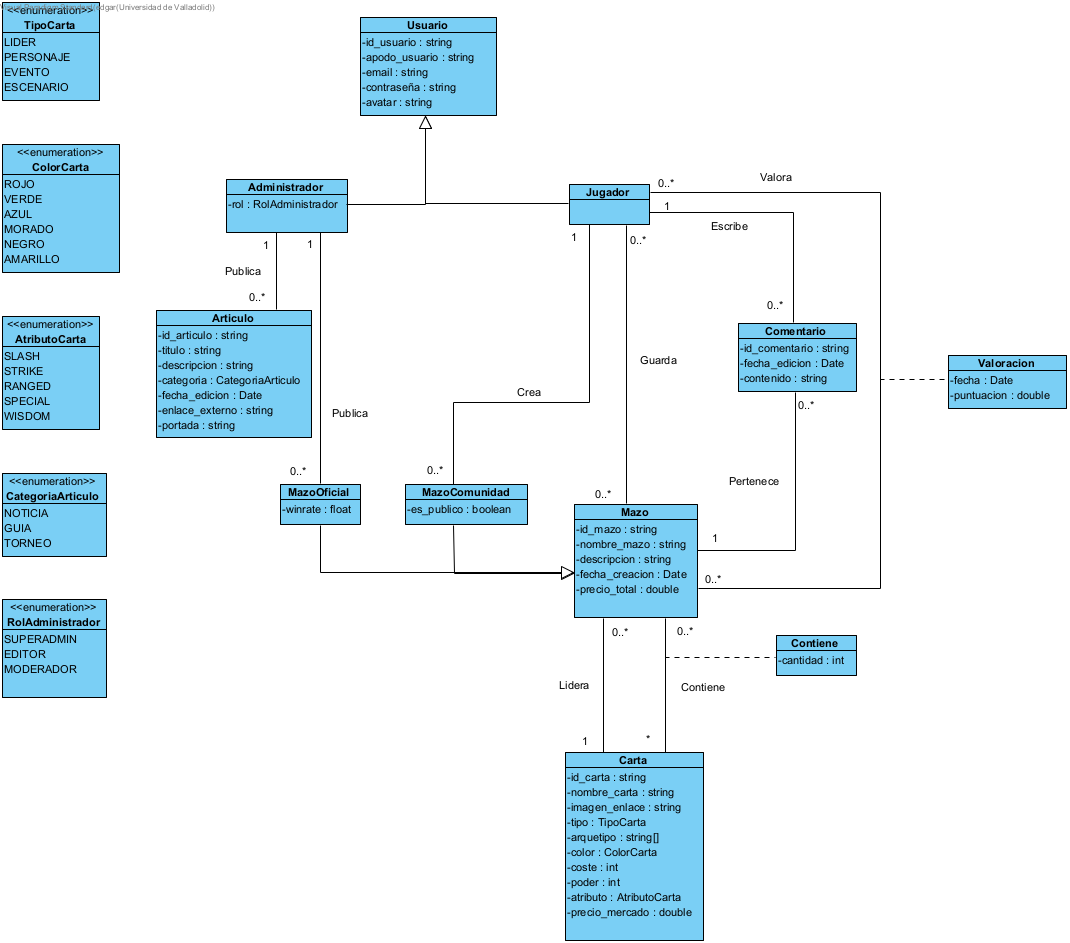
\includegraphics[width=0.9\textwidth]{Recursos/ModeloDominio_Grupo33v5.png}
		\caption{Diagrama UML del Modelo de Dominio de Card Partner}
		\label{fig:modelo_dominio}
	\end{figure}
	
	
	
	
	\newpage
	\section{Diseño del mapa del sitio web}
	\subsection*{Descripción del mapa del sitio web}
	El mapa del sitio web define la jerarquía de navegación y la reutilización de vistas y centralización de las herramientas. La estructura está diseñada para facilitar el acceso rápido a las diferentes herramientas de Card Partner a través de su menú de navegación en la barra superior de la página, disponible en cualquier momento.\\
	
	El mapa está estructurado en 4 niveles de profundidad para facilitar una entrada sencilla y estructurada a las herramientas:.\\
	\begin{itemize}
		\item \textbf{Nivel 0: Punto de entrada}\\
			El nivel 0 es la base de la estructura de la web, la \textbf{Página Principal} y es el punto de entrada de los usuarios. Desde ahí se muestra accesos rápidos a diferentes subsecciones de la web que pueden ser interesantes para usuarios nuevos o novedades para los usuarios experimentados.\\
		\item \textbf{Nivel 1: Navegación global}\\
			El nivel 1 es la base de la navegación dentro de la web. El \textbf{Menú de navegación} es la barra de navegación accesible en todo momento que divide la web en 4 grandes secciones, correspondientes al nivel 2 que son las herramientas para el usuario\\
		\item \textbf{Nivel 2: Herramientas y listados}\\
			El nivel 2 son las diferentes herramientas y visualización de contenido que ofrece la web a los usuarios, que se han dividido en 4 secciones:
			\begin{itemize}
				\item \textbf{SOCIAL:} Este apartado mostrará 3 subsecciones que llevarán al \textbf{Listado de Artículos} que mostrará contenidos de  categorías de artículos diferentes (Noticias, Guías o Torneos) según desde dónde se acceda, y haciendo click en el artículo se redirigirá al usuario al sitio externo referido del artículo.
				\item \textbf{CARTAS:} Este apartado llevará directamente al \textbf{Listado de cartas}, página donde se mostrarán las cartas del TCG y se podrá acceder a cada una de ellas, dirigiendo al \textbf{Visualizador de carta} que mostrará más información en detalle sobre la carta seleccionada.
				\item \textbf{MAZOS:} Este apartado agrupa las herramientas referidas a los mazos; el \textbf{Creador de mazos} que es la herramienta que permitirá al usuario crear su propio mazo eligiendo las cartas de la web, y el \textbf{Listado de Mazos}, que desde esta sección se podrá acceder a 2 contenidos distintos, \textbf{Listado de mazos comunidad} que son los mazos creados y publicados por los usuarios de la web y \textbf{Listado mazos META}, que son los mazos más recomendados en la actualidad por toda la comunidad de TCG por sus estadísticas.
				\item \textbf{USUARIO:} El apartado usuario se divide en 2 secciones en función si el usuario ha iniciado sesión o no.\\
				Si no ha iniciado sesión, se podrá crear un nuevo usuario o iniciar sesión con una cuenta registrada, lo que devolverá al usuario a la página en la que se encontrase con las nuevas funcionalidades posibles con sesión iniciada.\\
				Con la sesión iniciada, se mostrarán las secciones de \textbf{Gestión de Mi Cuenta} y las secciones de \textbf{Gestión de mazos creados}, \textbf{Gestión de mazos publicados} y \textbf{Gestión de mazos guardados}, que redirigirá al \textbf{Listado de Mazos} con los diferentes contenidos respectivamente, y a su vez podrá redirigir al \textbf{Creador de mazos} para editar los mazos del usuario.
				\item \textbf{TCG:} El apartado TCG mostrará la posible ampliación a futuro de la página web que cambiará el contexto del juego de cartas referido en toda la página.
			\end{itemize}
			
		\item \textbf{Nivel 3: Visualizadores y flujos verticales}\\
			El nivel 3 es el referido a los visualizadores mencionados que ofrecen el máximo detalle del contenido de la web, donde convergen los distintos listados de contenido del nivel 2 y flujos de navegación cruzada representados con líneas discontinuas. 
			\begin{itemize}
				\item \textbf{Visualizador de carta:} accesible desde el listado de cartas, muestra los detalles de una carta y ofrecerá redireccionamiento a una web externa oficial sobre la carta.
				\item \textbf{Visualizador del mazo:} Ofrece la lista de cartas e información adicional del mazo, además de direccionar al \textbf{Visualizador de carta} al seleccionar una carta del mazo para verla en más detalle o desde el mazo, poder ir al \textbf{Creador de mazos} con el contenido del mazo que está siendo visto para poder crear una copia y editar sus contenidos.
			\end{itemize}
	\end{itemize}
	
	\newpage
	\subsection*{Diagrama del mapa del sitio web}
	\begin{figure}[H]
		\centering
		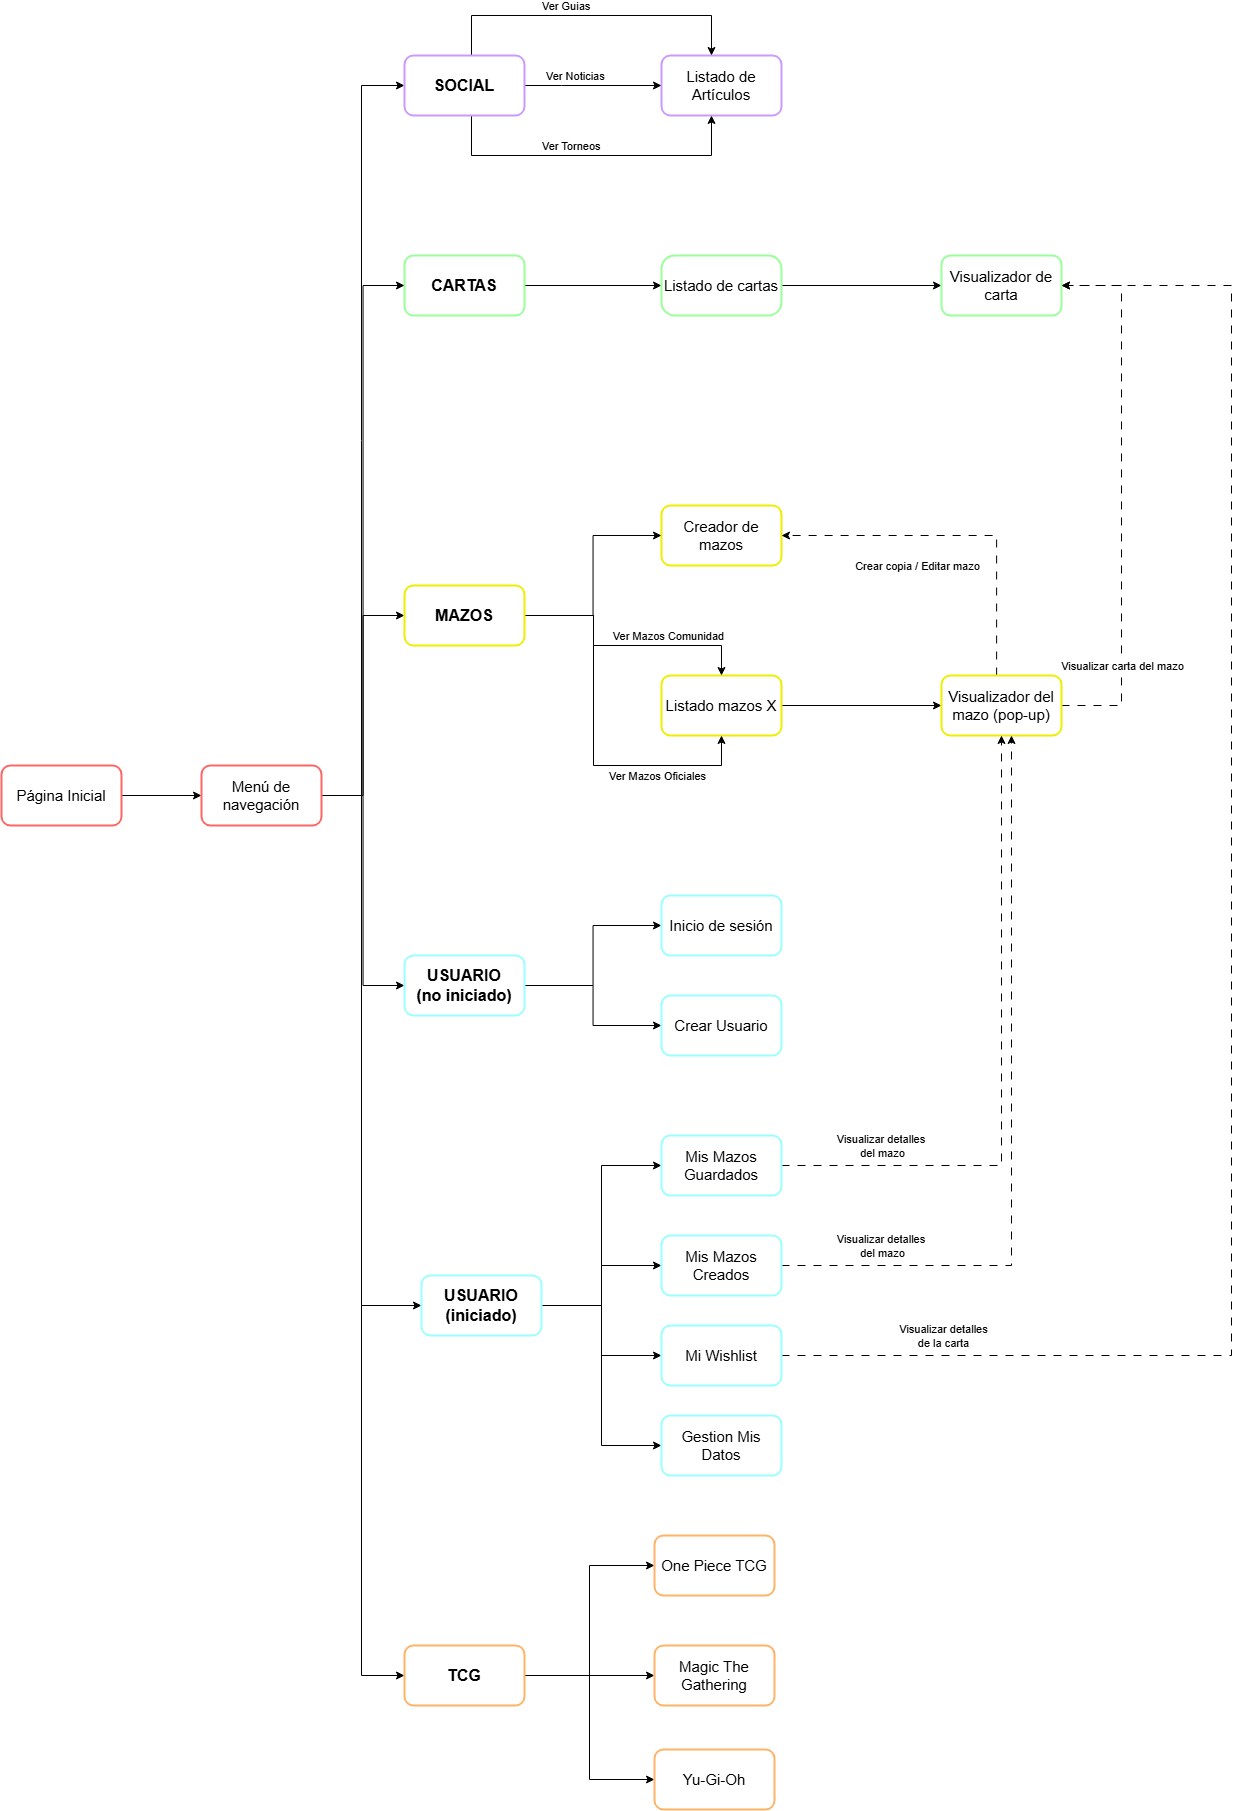
\includegraphics[width=1\textwidth]{Recursos/Mapa Card Partner v3.png}
		\caption{Estructura jerárquica y mapa del sitio web de Card Partner.}
		\label{fig:mapa_sitio}
	\end{figure}
	
	\subsection{Flujos de navegación}
		\subsubsection{Consulta de mazos}
			El usuario quiere consultar los mazos del META del TCG de One Piece.\\
			El usuario accede a la web a la \textbf{Página Inicial}, desde allí en el \textbf{Menú de navegación} se encontrará con varios desplegables, entre ellos \textbf{MAZOS} que mostrará varias opciones y una de las opciones será \textbf{Listado mazos META}.
			\begin{center}
				\textbf{Página Inicial} $\rightarrow$ \textbf{MAZOS} $\rightarrow$ \textbf{Listado mazos META}
			\end{center}
		\subsubsection{Consultar noticias}
		El usuario quiere informarse sobre las últimas novedades, expansiones o anuncios del juego.\\
		El usuario accede a la \textbf{Página Inicial}. En el \textbf{Menú de navegación}, accede desde el apartado \textbf{SOCIAL}, y al pulsar sobre la opción \textbf{Ver Noticias} el sistema le redirige al \textbf{Listado de Artículos(Noticias)}.
		\begin{center}
			\textbf{Página Inicial} $\rightarrow$ \textbf{SOCIAL} $\rightarrow$ \textbf{Ver Noticias} $\rightarrow$ \textbf{Listado de Artículos}
		\end{center}
			
		\subsubsection{Consulta de cartas}
		El usuario necesita buscar los detalles, el efecto o el precio de mercado actual de una carta específica.\\
		El usuario entra en la \textbf{Página Inicial} y selecciona \textbf{CARTAS} en el \textbf{Menú de navegación}. Esto le lleva al catálogo general, donde tras aplicar filtros y buscar la carta deseada, hace clic sobre ella para abrir una vista detallada con toda su información.
		\begin{center}
			\textbf{Página Inicial} $\rightarrow$ \textbf{CARTAS} $\rightarrow$ \textbf{Listado de cartas} $\rightarrow$ \textbf{Visualizador de carta}
		\end{center}
		
		\subsubsection{Consultar detalle de una carta desde un mazo}
		Mientras el usuario estudia la composición de una baraja, se encuentra con una carta que no conoce y necesita ver sus atributos, efectos o precio de mercado.\\
		El usuario se encuentra visualizando un mazo desde el \textbf{Visualizador del mazo}. Al hacer clic sobre una carta específica del listado, la web le redirigirá directamente la carta específica mediante el \textbf{Visualizador de carta}, sin tener que buscarla manualmente en el catálogo.
		\begin{center}
			\textbf{Página Inicial} $\rightarrow$ \textbf{MAZOS} $\rightarrow$ \textbf{Listado mazos X} $\rightarrow$ \textbf{Visualizador del mazo} $\rightarrow$ \textbf{Visualizador de carta}
		\end{center}
		
		\subsubsection{Navegación por guías de juego}
		Un usuario principiante quiere aprender las mecánicas básicas para iniciarse en el TCG de One Piece.\\
		El usuario accede a la \textbf{Página Inicial} y despliega el \textbf{Menú de navegación}. Se dirige a la sección \textbf{SOCIAL} y selecciona la opción \textbf{Ver Guías}. El sistema renderiza el \textbf{Listado de Artículos} filtrando la base de datos para mostrar únicamente el contenido de aprendizaje, permitiendo al usuario acceder a las explicaciones.
		\begin{center}
			\textbf{Página Inicial} $\rightarrow$ \textbf{SOCIAL} $\rightarrow$ \textbf{Ver Guías} $\rightarrow$ \textbf{Listado de Artículos}
		\end{center}
		
		
	\newpage
	\section{Cambios con respecto a la idea inicial}
		En este apartado comentaremos los cambios que hemos tenido con respecto a la idea incial
		\subsection{Torneos}
			Esta sección de la web estaba planteada para mostrar información de los torneo, esto supone, que un administrado tiene que estar mirando constantemente todos los torneos, ya sean locales, regionales o mundiales, para ir actualizando la vista de cada uno de ellos. \\ 
			Debido a la gran cantidad de los mismos, y  la dificultad para establecer un filtro de qué torneos en qué regiones son representativos hemos decidido aplicar un enfoque similar al apartado de notificas y de guías, tener enlaces a cada uno de los torneos, y para los winrates, tener esa información en el apartado de mazos meta, puesto que esta estadística, aporta una información mucho más útil de los mazos  de una manera más simple, permitiendo al usuario de un vistazo consultar qué mazos son META sin necesidad de tener que navegar por los diferentes torneos.
			
	\newpage
	\section{Reparto de carga de trabajo}
	Todos los integrantes hemos participado en todas las fases del trabajo y repartido el trabajo de forma equitativa, aunque encargándonos cada uno especialmente de alguna parte.\\
	
	\begin{table}[h]
		\centering
		\caption{Distribución de Responsabilidades por Miembro}
		\begin{tabularx}{\textwidth}{llX} 
			\toprule
			\textbf{Nombre} & \textbf{Porcentaje} & \textbf{Responsabilidad principal} \\
			\midrule
			ÁLVAREZ FULCONIS, MARCOS PALATINO      	& 25\%                & Diseño de las vistas tcg, social,noticias,torneo y guías\\
			LOPEZ PRIMO, ÁLVARO      				& 25\%                & Diseño del index, login y todas sus opciones, creación del repositorio de github, redacción del documento\\
			OTERO GARCÍA, SERGIO     				& 25\%                & Diseño de decks y todos sus submenús, \textit{comunity decks, meta decks}, creación de mazos,vista de cartas\\
			SANTIESTEBAN MENDO, EDGAR    			& 25\%                & Modelo de dominio,flujos de navegación, requisitos y redacción del documento\\
			\bottomrule
		\end{tabularx}
	\end{table}
	
	
	\section{Declaración de Uso de Inteligencia Artificial}
	Para esta segunda entrega, se ha usado la IA Gemini como herramienta para dudas y mejoras del archivo LaTeX, revisión de los contenidos y evaluación de los mismos y diseño iterativo para mejorar lo ya realizado.\\
	Además, se ha usado \href{https://gemini.google.com/share/7a923a0bfae8}{Gemini} para la generación del logo del proyecto.
	
	\textbf{Ejemplos de prompts realizados:}
	\begin{itemize}
		\item 'Cómo podemos realizar un menú desplegable en html a partir de un botón'
		\item 'Cómo podemos hcer un enlace en una imagen'
		\item 'Cómo podemos hacer un popup para cambiar la contraseña'
		\item 'Cómo funciona un hover en html'
		\item 'Redimensionar los botones para que ocupen una parte proporcional del encabezado'
		\item 'En css por qué me sale un link subrayado'
		\item 'Como puedo hacer un popup con sobreado'
		\item 'La estructura de un proyecto html cuál es'
		\item 'Entre la idea X y la idea Y, dime posibles ventajas y desventajas de cada uno y cuál se adaptaría mejor al proyecto y por qué'
	\end{itemize}
	
	%\begin{itemize}
	%   \item Herramientas utilizadas: hay que especificar qué herramientas de IA se han utilizado.
	%  \item Propósito del uso: explicar cómo se ha utilizado cada herramienta.
	% \item Alcance del uso: indicar en qué partes específicas del trabajo se ha recibido asistencia de una herramienta de IA.
	%\item Prompts utilizados: incluir los prompts, preguntas o instrucciones exactas que se han
	%introducido en la herramienta de IA.
	%\end{itemize}
	
\end{document}